%%%%%%%%%%%%%%%%%%%%%%%%%%%%%%%%%%%%%%%%%%%%%%%%%%%%%%%%%%%%%%%%%%%%%%%%
%                                                                      %
%     File: Thesis_Interface_FIFO.tex                        %
%     Tex Master: Thesis.tex                                %
%                                                                      %
%     Author: Carlos A. Rodrigues                         %
%     Last modified : 15 Abril 2013                         %
%                                                                      %
%%%%%%%%%%%%%%%%%%%%%%%%%%%%%%%%%%%%%%%%%%%%%%%%%%%%%%%%%%%%%%%%%%%%%%%

\chapter{Interface FIFO}
\label{chapter:Iter_FIFO}

Nas \ac{ACK} comdições iniciais do projecto seria o systema construido ser capaz de comunicar com dois modelos que seria acrescentados posteriormente ao sistema. Os dois modelos que serão ligados poderam ter frequencia de clock totalmente dististas do sistemas construido. Os modelos que se pretendem ligar são modelos simples que não têm disponível um processador, por essas razão este modelos querem escrever para o sistema que estamos a desenvolver sempre que têm dados, e ler sempre que são imformados que têm dados de leitura.   Por essa razão opetou-se por utilizar um sistema de comunicação simples e que trabalho-se de forma assíncrona. A comunidade Opensource ainda não tinha disponivel qualque cores desenvolvido ou mesmo começado. Por ser uma comunicação de forma simples, assincrona e onde era importante uma elevada de taxa de transferência de dados. Ponderou-se a utilização de duas memorias do tipo FIFO para cada modelo que se pretencia comunicar, onde seria utilizado uma fifo para cada sentido. Como pretendemos uma comunicação rápida entres o sistema e os modelos os dados serão enviados em paralelo permitindo assim uma redução bastante grande do tempo de envio de dados.

Como se pode ver na figura \ref{fig:ligacoesFIFO} este core tem disponível uma interface wishbone para comunicação com o processador do sistema e uma outra interface que utiliza 8 ligações de comunicação, sendo 2 delas de dados utilizando uma para cada sentido. As restantes linhas destinam-se para controlo informando o modelo lá ligado do estado do core. 

\begin{figure}[!htb]
  \centering
  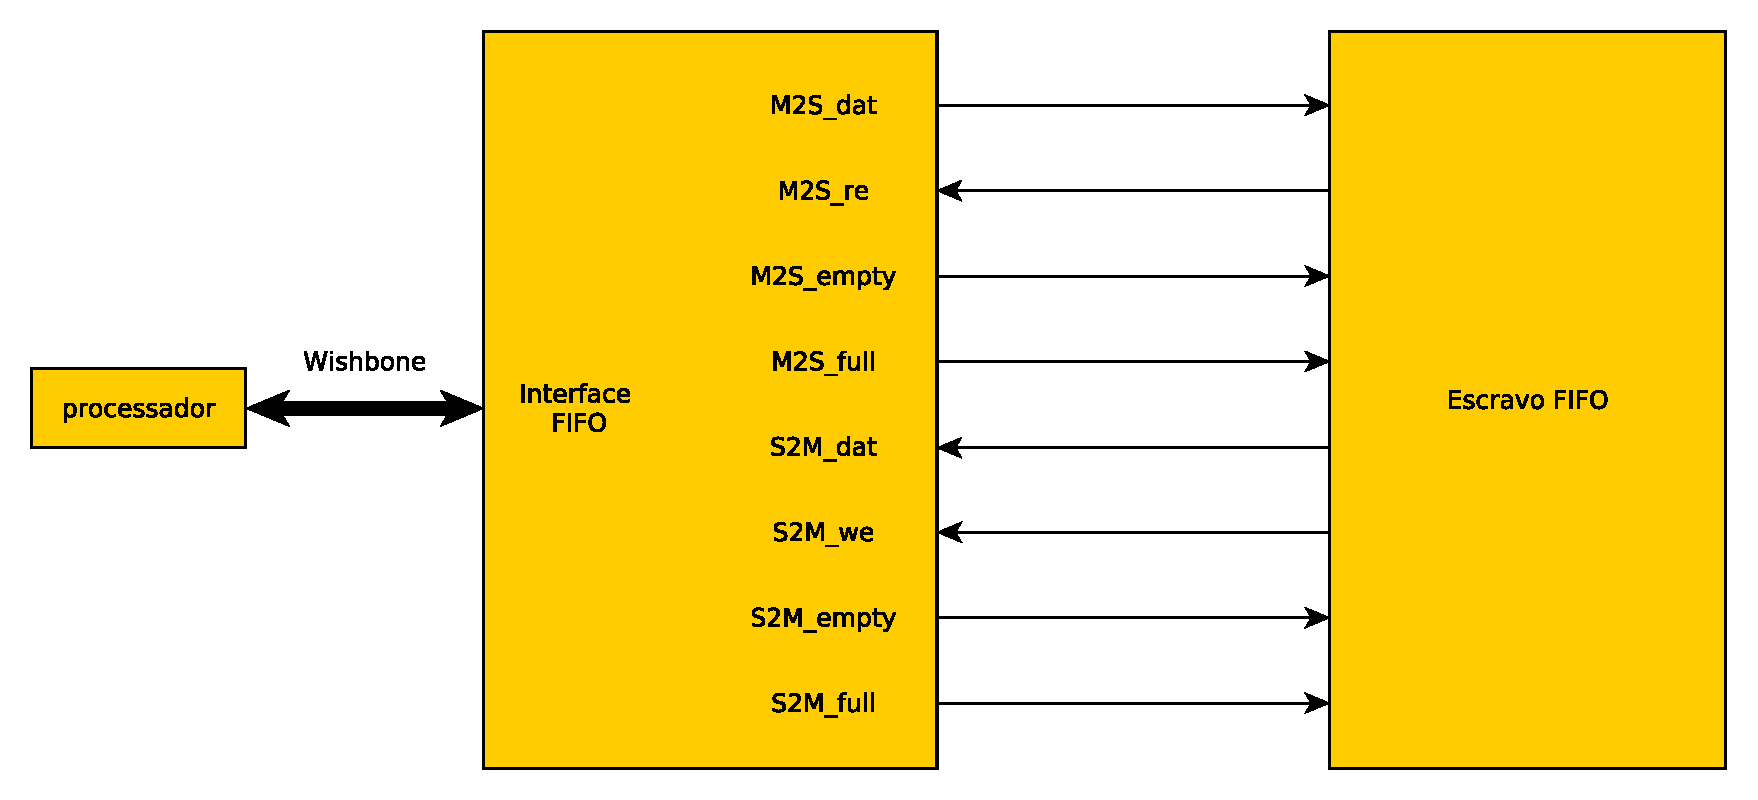
\includegraphics[width=0.75\textwidth]{grafos/FIFO.pdf} %1
  \caption[Protocolo FIFO]{Esquematico do sistema de comunicação FIFO.}
  \label{fig:ligacoesFIFO}
\end{figure}

Como já foi dito antes o core utilizada duas memorias FIFO para a gestão de dados para cada sentido como se pode ver na figura \ref{fig:fluxo_Interface FIFO}. Os dados que são enviado pelo wishbone são guardados na FIFO até o modelo que se encontra do outro lado pedir para o ler. Apenas assim o dados é enviado da memoria FIFO identificada na figura por M2S\_FIFO e envida para o modelo. Quando o modelo pretende enviar dados para o sistemas este envia os dados para a memoria FIFO na figura com o nome de S2M\_FIFO, os dados seram guardado na memorias até o processador pedir mais dados desta interface. O processador antes de enviar ou ler dados da interface deverá ver os estados da memoria correspondente, para o caso de querer enviar dados de verificar se a memoria numerada na figura por M2S\_FIFO não se encontra cheia, para não escrever em cima de dados validos. No caso de pretender ler deverá verificar se a memoria para esse efeito se têm dados, para não ler dados que não fazem sentido. Este procedimento também deverá ser feito pelos modelos que utilizam esta interface, para não haver problemas querencia. 

\begin{figure}[!htb]
  \centering
  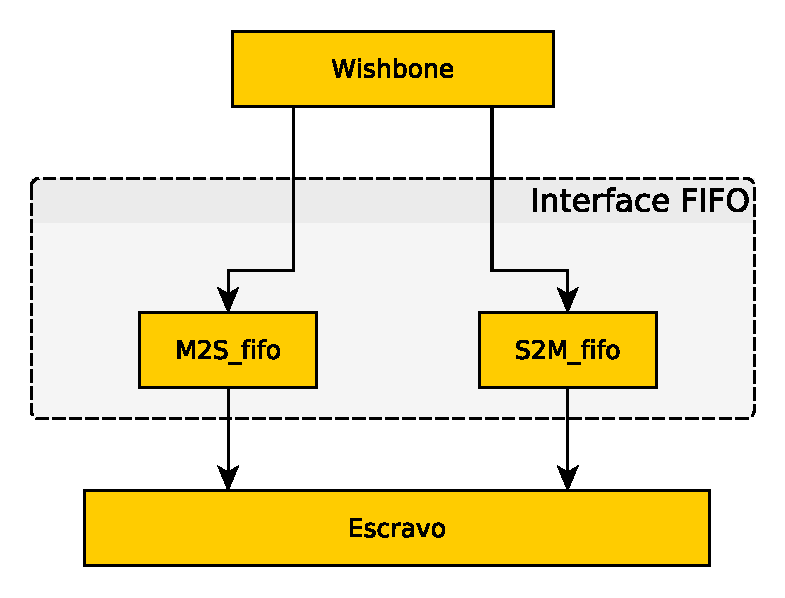
\includegraphics[width=0.50\textwidth]{grafos/diagrama_Interface_FIFO.pdf} % % mudar as setas desta figura.
  \caption[Fluxo de dados do core Interface FIFO]{Fluxo de dados do core Interface FIFO}  
  \label{fig:fluxo_Interface FIFO}
\end{figure}


O core tem dois grandes grupos de linhas de comunicação como se pode ver na tabela \ref{table:sinais_Interface_FIFO}, tem disponível todas as linhas de comunicação wishbone que se encontra ligada ao ao  e a parte de ligações relacionada com o controlo de dados enviados e recebidos pelo outro modelo. O processador pela interface Wishbone tem acesso a informações importantes sobre o cores relacionadas com o estado das duas memorias fifo, permitindo assim este saber quando poder ler dados validos e quando pode enviar dados sem perder dados. O conjunto de ligações da interface FIFO, onde seram ligados os modelos com que se pretendem comunicar.


Como se pode ver na tabela as primeiras quatro ligações são utilizadas para a recepçao e gestão dos dados do sistemas que seram enviados para o outro modelo. As outro quatro ligação são utilizadas para o sentido oposto ou seja para a comunicação e gestão do dados enviados do modelos para para o sistemas que estamos a desenvolver. As linhas identificadas por o sufixo "dat\_i" e "dat\_o" destinasse as ligações para a troca de dados, uma para para entrada de dados e outra para o envio de dados respectivamento, como esta interface é paralela esta duas linhas representam um conjunto de ligações que será do tamanho igual ao tamanho das palavras de dados que pretendemos enviar. Ou seja se pretendemos enviar palavras de 32 bits cada uma destas linhas tem um tamanho de 32 ligações.As linhas identificadas na figura pela sufixo empty e full, empty para vazia e full para cheia, são utilizadas para informar o outro modelo do estado das memorias FIFO's. A linha identificada na figura por M2S\_re é  utilizada pelo outro modelo para informar que está a ler a informação disponível da linha de dados. Por ultimo a linha na figura com o nome M2S\_we informa que os dados que estão na linha de dados de leitura são dados validos para guardar na memoria FIFO.



\begin{table}[h!]
  \begin{center}
    \begin{tabular}{|C{2cm}|c|c|c|}
      \hline
      Interface & Nome & direcção & Descrição \\
      \hline \hline
      \multirow{9}{*}{Wishbone} & clk\_i & input & Clock, Recebido pelo Wishbone. \\
      \cline{2-4}
      & rst\_i & input & Reset, renicia o core quando se encontra no valor logic "1".\\
      \cline{2-4}
	  & cyc\_i & input & \\
      \cline{2-4}
	  & stb\_i & input & \\
      \cline{2-4}
	  & adr\_i & input & Endereço do registo onde se pretende ler ou escrever no core.\\
      \cline{2-4}
	  & we\_i & input & Bit de selecção de escrita.\\
      \cline{2-4}
	  & dat\_i & input & Recepecção de dados por parte do processador.\\
      \cline{2-4}
      & dat\_o & output & Envio de dados para o processador.\\
      \cline{2-4}
      & ack\_o & output & bit que informaça o processador a recepecção do comando pelo core.\\
      \hline \hline
	  \multirow{8}{*}{FIFO} & fifo\_s2m\_dat\_i & input & sinal de entrada de dados do escravo para o mestre. \\
      \cline{2-4}
      & fifo\_s2m\_we & input & sinal de escrita do escravo. \\
      \cline{2-4}
      & fifo\_s2m\_empty & output & sinal da fifo que envia os dados do escravo para mestre se encontra vazia.\\
      \cline{2-4}
      & fifo\_s2m\_full & output & sinal da fifo que envia os dados do escravo para mestre se encontra cheia.\\
      \cline{2-4}
      & fifo\_m2s\_dat\_o & output & sinal de saida de dados do mestre para o escravo\\
      \cline{2-4}
      & fifo\_m2s\_re & input & sinal de leitura do escravo.\\
      \cline{2-4}
      & fifo\_m2s\_empty & output & sinal da fifo que envia os dados do mestre para escravo se encontra vazia.\\
      \cline{2-4}
	  & fifo\_m2s\_full & output & sinal da fifo que envia os dados do mestre para escravo se encontra cheia.\\
      \hline
    \end{tabular}
  \end{center}
  \caption[Tabela de sinais do core Interface FIFO]{Tabela de sinais da interface FIFO}
  \label{table:sinais_Interface_FIFO}
\end{table}

O core necessita de ter do lado do wishbone uma endereço como de pode ver na tabela \ref{table:registos_Interface_FIFO} esta tem apenas 2 endereço. o primeiro com um OFFset de 0X00 sendo o endereço de escrita de de leitura do dados para enviar e enviados pelo modelo. O segundo endereço com o OFFset de 0X02 é um endereço apenas de leitura é onde contem os dados das FIFO.

\begin{table}[h!]
  \begin{center}
    \begin{tabular}{|c|c|c|c|}
      \hline
      Nome & leitura/escrita & Descrição & Offset End. \\
      \hline \hline
      Leitura e escrita de dados& escrita e leitura & Envio ou rececção dos dados& 0X00 \\
      \hline
      Estado fifos & leitura & leitura dos estados das fifos& 0X02 \\
      \hline
    \end{tabular}
  \end{center}
  \caption[Tabela de registo do core Interface FIFO]{Tabela de registos da interface FIFO}
  \label{table:registos_Interface_FIFO}
\end{table}


Sempre e por qualquer das duas interfaces deverá ser feitar uma verificação dos dados na fifo. No caso da leitura da memoria FIFO deverá verificar-se que a memorias não está vazia e no caso da escrita verificar que esta não está cheia. Evitando-se assim no primeiro caso a ler-se dados errados e no segundo caso estar-se a escrever em cima de dados importantes e estes serem perdidos.